% Section content template for individual Educative lessons
% This file contains the actual content for a specific section
% Generated from Educative API section content

% Section: System Design: The Distributed Messaging Queue
% Section ID: 5148400467312640
% Section Slug: system-design-the-distributed-messaging-queue
% Generated: 2025-12-07T20:57:31.730188

\subsection{What is a messaging queue?}\label{GdGrUL_3DPOAVvNdffq0g}
\\
A \textbf{messaging queue} is an intermediate component that connects the interacting entities, known as \textbf{producers} and \textbf{consumers}.
\\
The producer \emph{produces} messages and places them in the queue, while the \emph{consumer} retrieves the messages from the queue and processes them. There may be multiple producers and consumers interacting with the queue simultaneously.
\\
Here is an illustration of two applications interacting via a single messaging queue:

\begin{figure}[htbp]
 \centering
 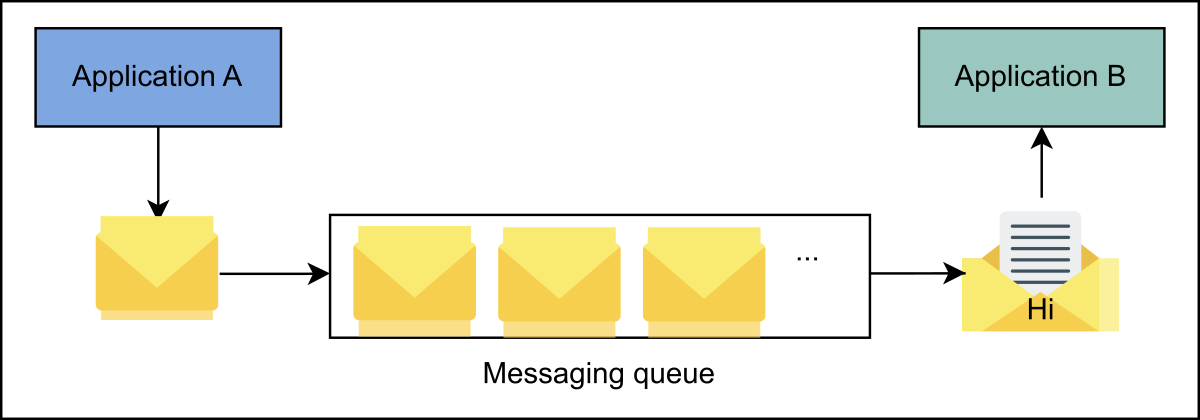
\includegraphics[width=0.5\textwidth]{Images/chapter_17/section_5148400467312640/5879464198406144.png}
 \caption{An example of two applications interacting via a single messaging queue}
\end{figure}

\subsubsection{Key components of a messaging queue}\label{Key-components}
\\
The key components of messaging queues include:
\\
\paragraph{Producers}\label{Producers}
\\
These are entities or applications that create and send messages to the queue. Producers generate data or events that need to be processed and push them into the messaging system for later consumption.
\\
\paragraph{Consumers}\label{Consumers}
\\
Consumers are entities or applications that receive and process messages from the queue. They subscribe to the queue and pull messages for processing, allowing them to handle tasks asynchronously and independently from the producers.
\\
\paragraph{Queues}\label{Queues}
\\
A queue is a data structure that temporarily holds messages sent by producers until they are consumed by consumers. Queues ensure that messages are stored in a first-in, first-out (FIFO) order, although some systems may implement different ordering mechanisms.
\\
They provide a buffer that decouples producers and consumers, allowing for smoother communication.
\\
\paragraph{Messages}\label{Messages}
\\
Messages are the data packets that are sent from producers to consumers via the queue.
\\
Each message typically contains a payload (the actual data) and metadata (such as headers or properties) that provide context about the message, such as its type, priority, or routing information. Together , these components enable efficient and reliable asynchronous communication in distributed systems, allowing for better resource management and improved system performance.
\\
Let\textquotesingle s discuss what advantages a messaging queue offers.

\subsection{Why use a messaging queue}\label{mXacg0QV42uY6eLkoRbVu}
\\
A messaging queue has several advantages and use cases.

\begin{itemize}
\item
\protect\phantomsection\label{1fOSScjCHeEa6B-5GD3On}
Messaging queues improve performance, reliability, scalability, and flexibility in distributed systems by enabling asynchronous, decoupled communication. Producers can send messages without waiting for consumers, reducing latency and preventing bottlenecks. Queues buffer messages during spikes or when consumers are offline, ensuring no data is lost and smoothing out load variations.
\item
\protect\phantomsection\label{08GqSQxTQxno_bKEyJkoK}
They also decouple services, allowing each component to operate, scale, deploy, and fail independently. This independence simplifies maintenance and fosters more agile development. Queues further support load balancing by distributing work across multiple consumers, automatically routing messages to available workers, and maintaining throughput even when some consumers slow down or fail.
\item
\protect\phantomsection\label{UjcXxRt7tqhCzWnbsmLmu}
Messaging systems enhance fault tolerance through persistence, retries, acknowledgments, and dead-letter queues, ensuring reliable delivery and easier troubleshooting. They make horizontal scaling straightforward---new consumers can be added at any time to increase processing capacity.
\item
\protect\phantomsection\label{7dNNmBQUoF8ErPNJhd1hn}
Additional benefits include rate limiting, where queues absorb bursts of traffic to protect downstream services, and priority handling, which ensures that critical work is processed first through multiple queues or priority rules.
\end{itemize}
\\
Overall, messaging queues provide a resilient, scalable backbone for modern applications, enabling smooth communication and consistent performance under varying loads.

\subsubsection{Common messaging queue patterns}\label{4_cvoRUOgPF9yHKcO0qOs}
\\
Point-to-point is a \emph{one-to-one} messaging pattern where a producer sends a message to a single consumer via a queue.
\\
Each message is delivered to exactly one designated consumer, making it ideal for tasks that must be handled by a specific worker. The queue tracks consumption and acknowledgments, ensuring guaranteed delivery. This model is commonly used in task queues and worker-based systems that need predictable, isolated processing.
\\
\textbf{Publish/subscribe (pub/sub or pub-sub)} is a \emph{one-to-many} pattern where a publisher sends messages to all subscribers interested in a topic, without knowing who they are.
\\
Because producers and consumers are decoupled, the system scales easily as subscribers join or leave. Publish /subscribe is widely used in event-driven architectures for real-time updates (such as newsfeeds and stock data) and notification systems where messages must reach multiple consumers simultaneously.

\begin{figure}[htbp]
 \centering
 
\includegraphics[width=0.15\textwidth]{Images/chapter_17/section_5148400467312640/6300499813203968.png}
 \caption{Pub/Sub}
\end{figure}

Request/reply supports \emph{synchronous, two-way} communication: a client sends a request and waits for a response. It 's used when immediate feedback is required, such as APIs, microservices, and transactional operations. Examples include checking product availability or orchestrating multiple services to fulfill a user request.
\\
This pattern improves user experience by providing timely, coordinated responses.

\begin{figure}[htbp]
 \centering
 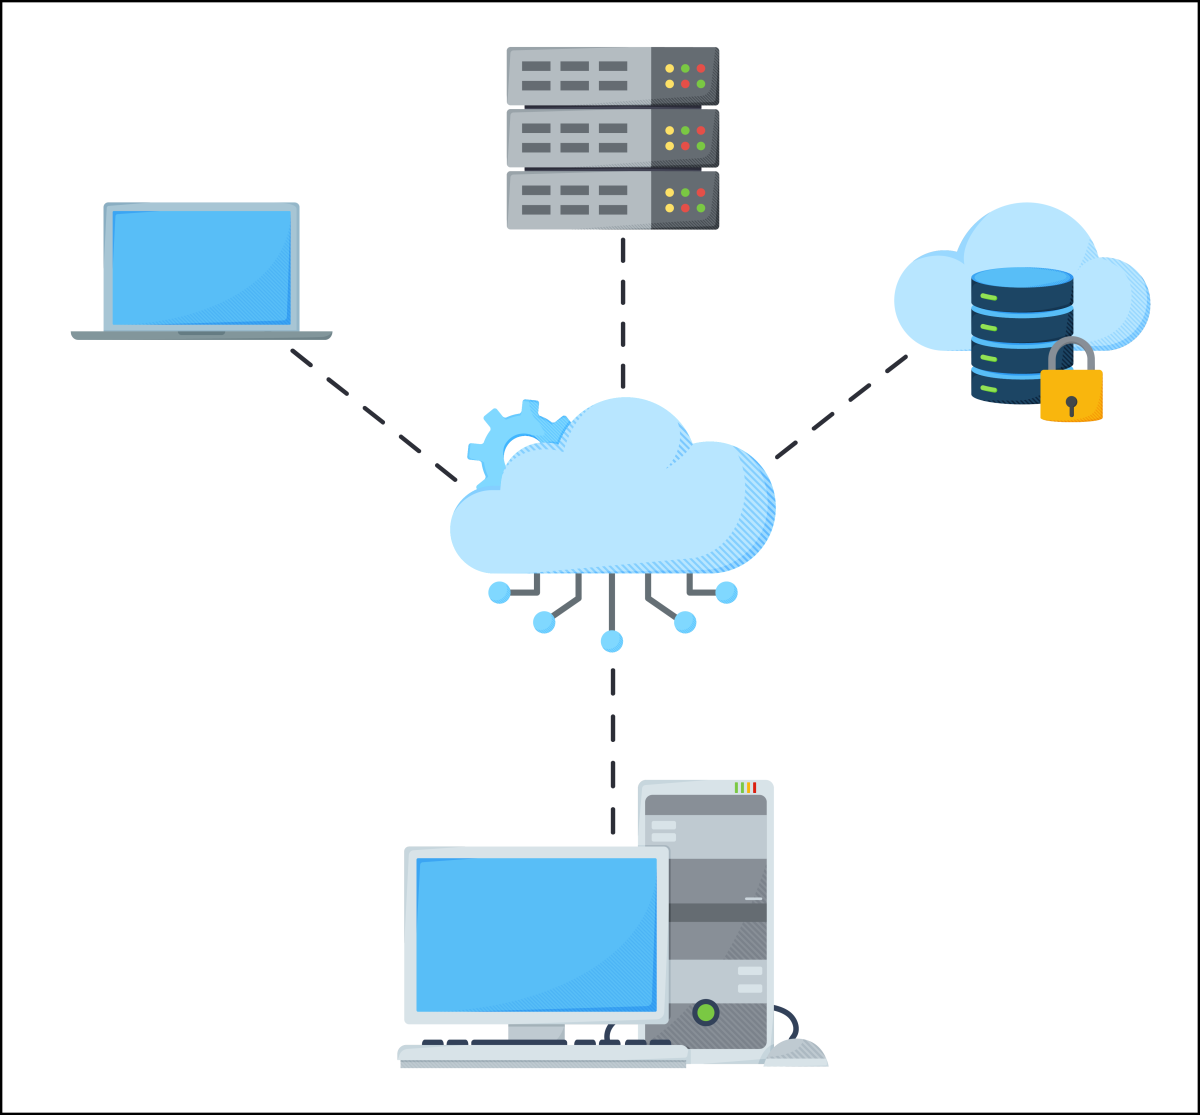
\includegraphics[width=0.25\textwidth]{Images/chapter_17/section_5148400467312640/5873963222040576.png}
 \caption{Point-to-point communication}
\end{figure}

\subsubsection{Popular messaging queue technologies}\label{HqeYQ37mz_ZFtRGvGuB1d}
\\
While the concept is universal, several popular technologies implement these principles, each with different strengths:

\begin{itemize}
\item
\protect\phantomsection\label{aCyoH-TEOzqxrT6MqqMq-}
\textbf{RabbitMQ:} A widely used open-source message broker that supports multiple protocols (like AMQP) and complex routing patterns.
\item
\protect\phantomsection\label{MqUHwoOV4UQg5wq3fX5cl}
\textbf{Apache Kafka:} A high-throughput, distributed streaming platform often used for real-time data pipelines, event sourcing, and log aggregation.
\item
\protect\phantomsection\label{yK85AWqKVhCc6OxkJkSmN}
\textbf{Amazon Simple Queue Service (SQS):} A fully managed message queuing service from AWS, offering reliable, scalable queues that integrate easily with other cloud services.
\end{itemize}
\\
Now, let's discuss the motivation behind designing a message queue.

\subsubsection{Messaging queue use cases}\label{lKLj3OwOmyPl8lbRWvvAo}
\\
A messaging queue has many use cases, both in single-server and distributed environments. For example, it can be used for interprocess communication within one operating system. It also enables communication between processes in a distributed environment.
\\
Some of the use cases of a messaging queue are discussed below.

\begin{enumerate}
\item
\protect\phantomsection\label{qzsvP7fTOzBRPcSsfht22}
\textbf{Sending many emails:} Emails are used for numerous purposes, including sharing information, account verification, password resets, marketing campaigns, and more. All of these emails, written for different purposes, don't need immediate processing and, therefore, don't disturb the system's core functionality. A messaging queue can help coordinate a large number of emails between different senders and receivers in such cases.
\item
\protect\phantomsection\label{tTOl85J5SfTbqe_-FpKRe}
\textbf{Data post-processing:} Many multimedia applications require processing content to meet the needs of different viewers, such as those for consumption on mobile phones and smart televisions. Oftentimes, applications upload the content into a store and use a messaging queue for post-processing of content offline. Doing this substantially reduces client-perceived latency and enables the service to schedule offline work at an appropriate time, probably late at night when compute capacity is less busy.
\item
\protect\phantomsection\label{TchH_Ib-WldJTMR-LGv4U}
\textbf{Recommender systems:} Some platforms utilize recommender systems to deliver personalized content or information to users. The recommender system takes the user's historical data, processes it, and predicts relevant content or information. Since this is a time-consuming task, a messaging queue can be incorporated between the recommender system and requesting processes to increase and quicken performance.
\end{enumerate}

\subsection{Best practices for implementing messaging queues}\label{l5ZkqNpOI0C1B82gBWXX1}

\subsubsection{Message idempotency}\label{OM3PB-YxQ9x8rwyEOF_wp}
\\
Message idempotency ensures that a message can be processed multiple times without causing duplicate actions or inconsistent data.
\\
This is particularly essential in distributed systems, where retries, failures, or network issues may result in duplicate deliveries. Idempotent design guarantees that reprocessing produces the same outcome as a single execution, simplifying error recovery and protecting data integrity.
\\
Overall, it strengthens system reliability and reduces the risk of unintended side effects.

\subsubsection{Monitoring and logging}\label{CaKvZz9s-2iYfvfTy9D4-}
\\
Monitoring and logging provide visibility into message flow and system health.
\\
Monitoring helps teams detect bottlenecks, latency spikes, and failures in real time, enabling proactive intervention. Logging captures key events and errors for auditing, troubleshooting, and determining the root cause of issues.
\\
Together, they improve operational transparency, support informed decisions, and enhance the resilience of messaging systems.

\begin{figure}[htbp]
 \centering
 
\includegraphics[width=0.15\textwidth]{Images/chapter_17/section_5148400467312640/5558680427036672.png}
 \caption{Error Handling}
\end{figure}

\subsubsection{Error handling}\label{4JrXrDnTBLc9EMk6zHuj3}
\\
Robust error handling ensures message processing continues smoothly even when failures occur.
\\
Common techniques include automatic retries for transient issues, dead-letter queues to isolate messages that repeatedly fail, and circuit breakers to prevent cascading failures. Combined with strong logging and monitoring, these strategies help teams diagnose problems, protect data, and maintain reliable system behavior.

\subsection{How do we design a distributed messaging queue?}\label{0zsPIcWFrm0pj3XPvIQZJ}
\\
We divide the design of a distributed messaging queue into the following five lessons:

\begin{enumerate}
\item
\protect\phantomsection\label{c-5qjrOsCCedZILD7ME_B}
\href{https://www.educative.io/courses/grokking-the-system-design-interview/requirements-of-a-distributed-messaging-queues-design}{\textbf{Requirements:}} In this lesson, we focus on the functional and non-functional requirements of designing a distributed messaging queue. We also discuss a single-server messaging queue and its drawbacks in this lesson.
\item
\protect\phantomsection\label{YhvJpDY1jwGbWir7c6ugq}
\href{https://www.educative.io/courses/grokking-the-system-design-interview/considerations-of-a-distributed-messaging-queues-design}{\textbf{Design}} \href{https://www.educative.io/courses/grokking-the-system-design-interview/considerations-of-a-distributed-messaging-queues-design}{\textbf{Consideration:}}~In this lesson, we discuss several important factors that may affect the design of a distributed messaging queue, including the order of placing messages in a queue, their extraction,~visibility in the queue, and the concurrency of incoming messages.
\item
\protect\phantomsection\label{aFo2iX_RVCD_GnLuoYsNU}
\href{https://www.educative.io/courses/grokking-the-system-design-interview/design-of-a-distributed-messaging-queue-part-1}{\textbf{Design:}} In this lesson, we examine the design of a distributed messaging queue in detail. We also describe the process of replication of queues and the interaction between various building blocks involved in the design.
\item
\protect\phantomsection\label{VwscFyBtJt-zza7_CxhaK}
\href{https://www.educative.io/courses/grokking-the-system-design-interview/evaluation-of-a-distributed-messaging-queues-design}{\textbf{Evaluation:}} In this lesson, we evaluate the design of a distributed messaging queue based on its functional and non-functional requirements.
\item
\protect\phantomsection\label{KqiluM22Gr2JkAlmreYTV}
\href{https://www.educative.io/courses/grokking-the-system-design-interview/quiz-on-the-distributed-messaging-queues-design}{\textbf{Quiz:}} At the end of the chapter, we assess your understanding of the design of a distributed message queue through a quiz.
\end{enumerate}
\\
Let's start by understanding the requirements of designing a distributed messaging queue.

% End of section content